\chapter{Informační systém pro správu závěrečných prací}

Téma bakalářská práce se zaměřuje na analýzu, návrh a~implementaci informačního systému pro správu bakalářských a~diplomových prací. Informační systém slouží především firmě Red Hat jako nástroj pro zadání, kontrolu a~schvalování závěrečných prací vypsaných na partnerských fakultách. Systém zároveň poskytuje rozhraní pro studenty, kteří se mohou přihlašovat k~tématům, komentovat jednotlivá témata a~závěrečné práce. Dále k~systému přistupuje vedoucí, který schvaluje přihlášení k~tématům a~spravuje stav závěrečných prací. Systém je veřejný a~návštěvníci tak mají možnost procházet jednotlivá témata a~závěrečné práce, dále se mohou registrovat na základě fakultního e-mailu. Hlavní strana systému slouží jako přehled nejnovějších aktivit v~systému.

Mým úkolem je vytvořit grafickou podobu uživatelského rozhraní a tento návrh integrovat do systému.

\section{Popis požadavků na systém}

Systém eviduje---

\begin{itemize}
    \item Témata
    \item Závěrečné práce
    \item Uživatele
    \item Univerzity
    \item Přihlášky
\end{itemize}

Témata popisují cíl práce, mohou být vypsány pro více studentů. Systém umožňuje témata vypisovat, editovat a mazat. Témata evidují---

\begin{itemize}
    \item Seznam přihlášených studentů
    \item Seznam univerzit, na kterých je téma vypsáno
    \item Seznam vedoucích
    \item Seznam závěrečných prací, které byly na základě tématu vypsány
\end{itemize}

Ke každé závěrečné práci se smí přihlásit pouze jeden student. Systém umožňuje práce vytvářet (na základě tématu), editovat a mazat. Každá závěrečná práce eviduje---

\begin{itemize}
    \item Studenta přihlášeného k práci
    \item Téma, ze kterého byla práce vypsána
    \item Univerzitního vedoucího práce
    \item Typ závěrečné práce -- bakalářka nebo diplomka
    \item Stav závěrečné práce -- přihlášená, dokončená, neúspěšná a odložená
\end{itemize}

V systému tak existuje několik uživatelských rolí, které se liší v přístupových právech. Každý registrovaný uživatel je automaticky student. Práva uživatelských rolí---

\begin{itemize}
    \item Návštěvníci -- mohou procházet jednotlivá témata, závěrečné práce a registrovat se dle fakultního e-mailu.
    \item Studenti -- mohou se přihlašovat k tématům, spravovat vlastní závěrečné práce a diskutovat k jednotlivým tématům a závěrečným pracím.
    \item Univerzitní vedoucí -- jedná se o vedoucího na dané univerzitě, může vytvářet závěrečné práce, schvaluje přihlášky a má právo přispívat v diskuzích.
    \item Vedoucí -- na rozdíl od univerzitního vedoucího navíc vytváří témata závěrečných prací.
    \item Správce -- může spravovat většinu obsahu, přidávat univerzity a uživatele.
\end{itemize}

\section{Analýza cílové skupiny}

Cílová skupina uživatelů přistupujících k systému je velmi úzce zaměřená. Největší část návštěvníků tvoří studenti z technicky zaměřených oborů. Tato skupina je dána typem závěrečných prací, pro které je systém primárně určen---jedná se o témata z IT oboru. Příklady některých univerzit, které jsou v systému registrovány---

\begin{itemize}
    \item Masarykova univerzita
    \item Vysoké učení technické v Brně
    \item České vysoké učení technické v Praze
\end{itemize}

Systém je určen především pro studenty v posledních ročnících bakalářského nebo magisterského studia a jejich vedoucí.

\section{Základní layout}

Rozhodl jsem se používat tři základní layouty stránky, přičemž dva se liší pouze prohozením postranního panelu a obsahové části. Primární layout (viz obrázek \ref{img:layout1}) tvoří---

\begin{itemize}
    \item Navigační panel -- nachází se v záhlaví stránky a obsahuje hlavní informace o přihlášeném uživateli, vyhledávač a logotyp.
    \item Navigační menu -- slouží jako primární navigace na stránce.
    \item Levý sloupec s hlavním obsahem -- je určený pro seznam témat, závěrečných prací a jejich popis. Dále může obsahovat odevzdávárnu souborů a komentáře.
    \item Pravý sloupec s vedlejším obsahem -- slouží jako přehled informací o daném tématu nebo závěrečné práci. Dále může obsahovat nástroje pro správu témat (popř. závěrečných prací) nebo filtry.
\end{itemize}

Sekundární layout představuje kostru uživatelského profilu a profilu univerzity. Na rozdíl od primárního layoutu je sloupec s vedlejším obsahem přemístěn na levou část stránky. Tvoří ho---

\begin{itemize}
    \item Navigační panel
    \item Navigační menu
    \item Levý sloupec s vedlejším obsahem -- obsahuje podrobnější informace o uživateli včetně profilového obrázku.
    \item Pravý sloupec s hlavním obsahem -- slouží jako obecný přehled vedených závěrečných prací, vlastních prací a aktivity uživatele v systému.
\end{itemize}

Poslední layout je speciálně navržený pro formuláře. Obsahuje pouze nejnutnější elementy a je tvořen z jednoho sloupce---

\begin{itemize}
    \item Navigační panel
    \item Hlavní sloupec -- určený pro formulářová pole.
\end{itemize}

\begin{figure}[htbp]
    \centering
    \includegraphics[width=\textwidth]{images/main-layout.png}
    \caption{Drátěný model profilu zadání bakalářské nebo diplomové práce.}
    \label{img:layout1}
\end{figure}

Minimální šířka všech stránek je 1040$px$ -- při nižších hodnotách je uživatel nucen horizontálně skrolovat. Tuto šířku jsem zvolil s ohledem na aktuální podíl populárních rozlišení u displejů zařízení, který v současnosti z více než 90\% tvoří rozlišení větší než 1024$\times$768$px$\footnotemark[1].

\footnotetext[1]{\url{http://gs.statcounter.com/\#resolution-CZ-monthly-201203-201303}}

\section{Grafický návrh}

Přesto, že nebyly kladeny žádné větší nároky na dodržení vizuálního stylu společnosti Red Hat, rozhodl jsem se z něj čerpat alespoň částečně především co se týče barevnosti.

\subsection{Písmo}

Ještě relativně nedávno byly designeři při volbě písma pro webové aplikace omezeni na několik málo základních fontů, které byly ve většině případů přítomny na klientských počítačích -- například Arial, Times New Roman, Georgia nebo Courier Sans. Díky nového CSS pravidla \texttt{@font-face} je možné používat i fonty, které nejsou na klientských počítačích nainstalovány.

Již na počátku tvorby jsem se rozhodl používat pro nadpisy lineárně serifové písmo s rovnými serify\footnotemark[1]. Volba písma je značně omezená především pro nutnost podpory české znakové sady. První volbou bylo písmo Sanchez\footnotemark[2], které jsem však později zavrhl z důvodu špatné optimalizace pro webové prohlížeče. Nakonec jsem zvolil písmo Museo Slab\footnotemark[3], které navrhl designer Jan Buivenga.

\footnotetext[1]{Viz klasifikace písma podle Jana Solpery.}
\footnotetext[2]{\url{http://www.myfonts.com/fonts/latinotype/sanchez/}}
\footnotetext[3]{\url{http://www.myfonts.com/fonts/exljbris/museo-slab/}}

\begin{figure}[htbp]
    \centering
    \includegraphics[width=\textwidth]{images/museo.pdf}
    \caption{Museo Slab 500}
    \label{img:museo}
\end{figure}

Jako primární písmo jsem se rozhodl použít velmi rozšířený Arial. Jedná se o bezpatkový grotesk, který je již od počátku součástí všech verzí Microsoft Windows. Arial bývá často kritizován pro svou podobnost s Helveticou, přesto se však jedná o velmi dobře čitelný a vysoce optimalizovaný font.

\subsection{Piktogramová řada}

Jako sadu ikonek jsem zvolil Font Awesome\footnotemark[1], který byl primárně navržený pro webový rámec Twitter Bootstrap. Samotná piktogramová řada je vedena pod licencí CC BY 3.0, je tedy možné používat řadu samostatně.

\footnotetext[1]{\url{http://fortawesome.github.io/Font-Awesome}}

\subsection{Typografie}

Jako základní velikost písma jsem zvolil 16$px$, díky čemuž je text dobře čitelný i na monitorech s hustším PPI. Vzhledem k větší střední výšce písma Arial jsem se rozhodl použít vyšší hodnotu řádkového prokladu, aby i rozsáhlejší části textu nepůsobily příliš sevřeně.

Nadpisy první až čtvrté úrovně jsou vysázeny písmem Museo Slab s maximální velikostí 34$px$, která je užita výhradně pro názvy témat a závěrečných prací.

Velikost okrajů primárního sloupce s obsahem jsem se rozhodl nastavit na 30$px$, čímž je zajištěn dostatečný prostor pro jednoduchou orientaci mezi odstavci a jsou tak jasně odlišeny bloky textu.

\subsection{Barevnost}

Vizuální styl společnosti Red Hat se orientuje v barvách bílé, černé a červené. Rozhodl jsem se použít světlejší barvy pro navození klidnějšího dojmu a snížení kontrastu, neboť příliš vysoký kontrast může působit dráždivě a není podle mě příliš vhodný pro stránky určené primárně pro správu závěrečných prací.

V grafickém návrhu používám osm stupňů šedi a dva stupně červené barvy. Několik dalších barev je použito výjimečně například pro zvýraznění aktivních kategorií nebo pro systémové zprávy a upozornění.

\begin{figure}[htbp]
    \centering
    \includegraphics[width=\textwidth]{images/barvy.pdf}
    \caption{Základní barvy použité v uživatelském rozhraní.}
    \label{img:colors}
\end{figure}

\begin{figure}[htbp]
    \centering
    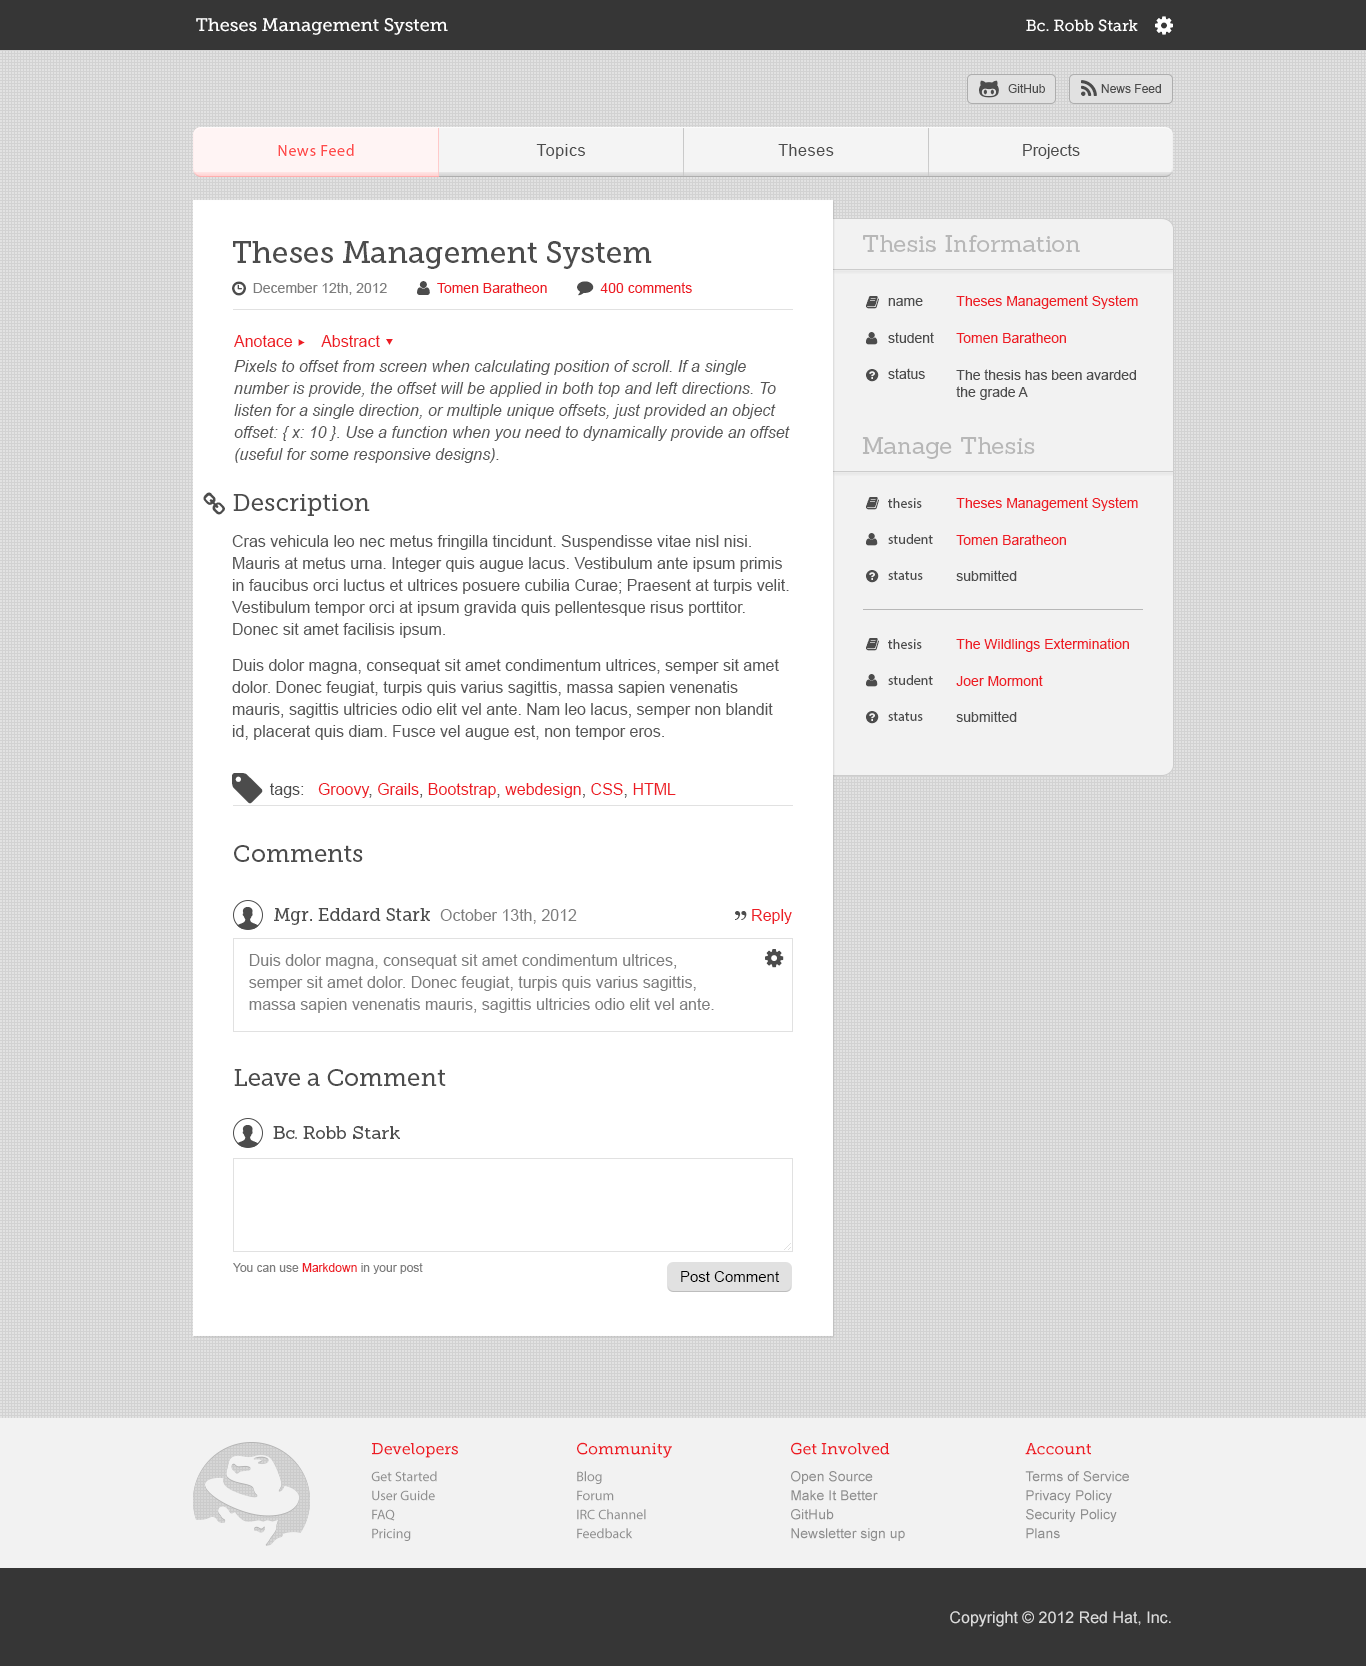
\includegraphics[width=\textwidth]{images/design.png}
    \caption{Výsledný grafický návrh -- profil bakalářské práce.}
    \label{img:design}
\end{figure}

\section{Kódování šablon}

Hlavní funkce systému jsou napsané v programovacím jazyce Groovy za použití platformy Grails. Výchozí jazyk této platformy pro popis prezentační vrstvy systému je GSP (\textit{Groovy Server Pages}), což je jazyk značně inspirovaný JSP (\textit{JavaServer Pages}) speciálně navržený pro dynamické zpracování HTML dokumentů. Syntaxe GSP vychází z XML, nejedná se však o XML validní dokumenty.

Dále jsem v systému použil Twitter Bootstrap, díky kterému je návrh jednotlivých HTML dokumentů konzistentní a lépe udržovatelný. Zároveň je tak docíleno vyšší podpory webovými prohlížeči, přičemž jsou dodržovány osvědčené postupy a doporučení.

Prezenční vrstva systému využívá následující technologie, knihovny a webové rámce:

\begin{itemize}
    \item HTML~5 (viz kapitola~\ref{sec:html})
    \item CSS~3 (viz kapitola~\ref{sec:css})
    \item LESS (viz kapitola~\ref{sec:less})
    \item JavaScript\footnotemark[1]
    \item Twitter Bootstrap (viz kapitola~\ref{sec:bootstrap})
    \item Groovy Server Pages
\end{itemize}

Zatímco ve čtvrté kapitole jsem se věnoval specifikaci těchto technologií, nyní se zaměřím na jejich použití v našem systému. Vzhledem k zaměření systému však není potenciál některých technologií plně využit (jde především o HTML~5 standard).

\footnotetext[1]{JavaScript je skriptovací dynamicky typovaný jazyk určen primárně pro rozšíření HTML dokumentu o dynamické chování na straně klienta.}

\section{HTML stránky}
\section{Kaskádové styly}
